\pdfoutput=1
\documentclass[11pt]{article}
\usepackage[utf8]{inputenc}
\usepackage[T1]{fontenc}
\usepackage{textcomp}
\usepackage{mathpazo}
\usepackage{microtype}
\usepackage[margin=1in]{geometry}
\usepackage{amsmath,amssymb}
\usepackage{graphicx}
\graphicspath{{figures/}{../figures/}}
\setkeys{Gin}{keepaspectratio}
\usepackage{longtable,booktabs,array,calc}
\usepackage{float}
\floatplacement{figure}{H}
\usepackage{caption}
\captionsetup{font=small,labelfont=bf}
\usepackage{needspace}
\usepackage{setspace}
\setstretch{1.1}
\usepackage{fancyhdr}
\usepackage{etoolbox}
\usepackage{upquote}
\usepackage[hyphens]{xurl}
\usepackage[colorlinks=true,linkcolor=blue,urlcolor=blue,citecolor=blue]{hyperref}
\usepackage{bookmark}

% Characters pdfLaTeX does not define by default.
\DeclareUnicodeCharacter{2212}{\ensuremath{-}}
\DeclareUnicodeCharacter{0394}{\ensuremath{\Delta}}
\DeclareUnicodeCharacter{03B1}{\ensuremath{\alpha}}
\DeclareUnicodeCharacter{03B2}{\ensuremath{\beta}}
\DeclareUnicodeCharacter{03BB}{\ensuremath{\lambda}}
\DeclareUnicodeCharacter{03C3}{\ensuremath{\sigma}}
\DeclareUnicodeCharacter{2208}{\ensuremath{\in}}
\DeclareUnicodeCharacter{2248}{\ensuremath{\approx}}
\DeclareUnicodeCharacter{221D}{\ensuremath{\propto}}
\DeclareUnicodeCharacter{2264}{\ensuremath{\leq}}
\DeclareUnicodeCharacter{2265}{\ensuremath{\geq}}
\DeclareUnicodeCharacter{2192}{\ensuremath{\rightarrow}}

% Macros used by pandoc's LaTeX output.
\providecommand{\tightlist}{\setlength{\itemsep}{0pt}\setlength{\parskip}{0pt}}
\makeatletter
\def\fps@figure{H}
\makeatother
\setlength{\emergencystretch}{3em}
\sloppy
\AtBeginEnvironment{longtable}{\footnotesize}

\hypersetup{pdftitle={When Validation Changes the Answer: GARCH(1,1) versus Gradient Boosting for Forecasting S&P 500 ETF Volatility}, pdfauthor={Muhammad Mateen Iqbal}}

\pagestyle{fancy}
\fancyhf{}
\fancyhead[L]{\small When Validation Changes the Answer}
\fancyhead[R]{\small Muhammad Mateen Iqbal}
\fancyfoot[C]{\thepage}
\renewcommand{\headrulewidth}{0.4pt}

\title{When Validation Changes the Answer: GARCH(1,1) versus Gradient Boosting for Forecasting S\&P 500 ETF Volatility}
\author{Muhammad Mateen Iqbal\\[2pt]
  {\normalsize BS Data Science, Institute of Computing \& IT, University of Lakki Marwat, Pakistan}\\
  {\normalsize\texttt{muhammadmateen1024@gmail.com}}}
\date{October 2026\\[2pt] {\small Code and data: \url{https://github.com/mateeniqbal3/vol-forecast-model-comparison}}}

\begin{document}
\maketitle
\thispagestyle{empty}

\begin{abstract}
This study asks whether a gradient-boosted tree model (LightGBM) forecasts
the 5-day realized variance of SPY better than GARCH(1,1) and a RiskMetrics
EWMA. It also asks whether the answer depends on how the models are
validated. All three models are scored under a naive random split of
forecast dates and under expanding-window walk-forward validation (26
annual folds, 2000--2025, 6,534 forecast dates). The walk-forward scheme
purges training targets that overlap the test period. The ML design, the
walk-forward protocol and the significance test were each fixed before the
results that could have influenced them.

Under walk-forward validation, LightGBM's QLIKE advantage over GARCH(1,1)
is 0.0124, which is not significant: Diebold--Mariano p = 0.47, 95\% CI
−0.046 to +0.022. Its RMSE is higher (1.589e-3 vs.~1.443e-3; p = 0.18).
Under the naive split the same model appears to beat GARCH decisively on
both losses (QLIKE p \textless{} 0.0001; MSE p = 0.016). On identical test dates the
naive split overstates LightGBM's QLIKE by 0.065 and GARCH's by 0.008; for
EWMA, which estimates nothing, it changes nothing.

The mechanism is identified directly. A tree ensemble's forecast is capped
by the targets it was trained on. The model trained through 2007 cannot
forecast above 0.0022 (about 33\% annualized volatility) for any input,
while the autumn of 2008 realized up to 0.035 (about 133\%). That one year
moves the full-sample QLIKE difference by +0.027, more than twice
LightGBM's net advantage. The added complexity was not justified, and
naive validation would have concluded the opposite.

\medskip
\noindent \textbf{Keywords:} volatility forecasting, GARCH, gradient boosting, LightGBM,
walk-forward validation, data leakage, QLIKE, Diebold--Mariano test,
pre-registration

\noindent \textbf{JEL classification:} C52, C53, C58, G17
\end{abstract}

\hypertarget{introduction}{%
\section{Introduction}\label{introduction}}

Machine-learning models are routinely proposed as improvements on
parametric volatility models. The comparison is easy to get wrong in two
ways. The first is validation: volatility is persistent, and forecast
targets built from overlapping windows are serially dependent. A random
train/test split therefore places training observations immediately next
to, and partly inside, the test observations. The second is selection:
when many designs are tried and the best one is reported, even a correct
validation scheme overstates out-of-sample performance.

This study compares a simple and a complex volatility forecaster under
controls for both problems, and reports the result together with the
answer a naive analysis would have given. Its contributions are modest and
specific:

\begin{enumerate}
\def\labelenumi{\arabic{enumi}.}
\tightlist
\item
  \textbf{A controlled contrast of validation schemes.} The naive and
  walk-forward forecasts of each model are scored on the same 1,321
  dates. This isolates the effect of the validation scheme from the
  effect of the sample period. The naive split's bias grows with how much
  a model learns from individual target rows: 0 for EWMA, 0.008 QLIKE for
  GARCH(1,1), 0.065 for LightGBM.
\item
  \textbf{A pre-registered comparison.} The design of the complex model, the
  walk-forward protocol and the significance test with its decision rule
  were each written down and committed before the results they could have
  influenced. Exactly one ML configuration was built and evaluated.
\item
  \textbf{A directly measured mechanism.} The walk-forward failure of the tree
  model is traced to a forecast ceiling. Scaling the model's variance
  inputs by 100 leaves its forecast unchanged.
\end{enumerate}

The finding echoes Hansen and Lunde (2005), who found little that
outperforms GARCH(1,1) for exchange-rate volatility. It does so for a
modern ML competitor, and with an explanation of \emph{why} the competitor falls
short.

\hypertarget{related-work}{%
\section{Related work}\label{related-work}}

\textbf{Parametric volatility models.} GARCH (Engle, 1982; Bollerslev, 1986)
and the exponentially weighted moving average of RiskMetrics (J.P. Morgan
and Reuters, 1996) are the standard benchmarks. Andersen and Bollerslev
(1998) showed that the apparently poor fit of GARCH forecasts largely
reflects the noise in squared-return proxies, not a failure of the model.
Hansen and Lunde (2005) compared 330 ARCH-type models and found little
evidence that any beats GARCH(1,1) for exchange-rate data. The HAR model of
Corsi (2009) motivates the multi-horizon realized-variance features used
here.

\textbf{Evaluation with a noisy proxy.} Patton (2011) showed that when forecasts
are compared against a conditionally unbiased but noisy variance proxy,
only certain losses rank them consistently. MSE and QLIKE on the variance
scale are among them; RMSE on the volatility scale is not. This study
therefore evaluates everything in variance units. Diebold and Mariano
(1995) provide the test of equal predictive accuracy, with
heteroskedasticity- and autocorrelation-consistent variance estimation
(Newey and West, 1987, 1994).

\textbf{Machine learning and financial validation.} Gradient boosting (Friedman,
2001), in the LightGBM implementation (Ke et al., 2017), is a common
default for tabular prediction. López de Prado (2018) stresses that
cross-validation on financial data leaks information through overlapping
labels and must be purged. Recent studies apply ML to volatility forecasting
with intraday data (e.g.~Christensen, Siggaard and Veliyev, 2023). This
study works at the daily frequency that free data allow, and puts its
emphasis on validation and pre-registration rather than on model breadth.

\hypertarget{data-and-forecasting-target}{%
\section{Data and forecasting target}\label{data-and-forecasting-target}}

\textbf{Data.}

\begin{itemize}
\tightlist
\item
  \textbf{Source:} daily split- and dividend-adjusted OHLCV for the SPDR S\&P
  500 ETF (SPY), from \texttt{yfinance}.
\item
  \textbf{Sample:} its first trading day (1993-01-29) to 2025-12-31, giving
  8,287 daily log returns.
\item
  \textbf{Cleaning:} no rows had duplicate dates or missing closes, so none
  were dropped.
\item
  \textbf{Drift check:} a data manifest records checksums of the return series,
  so a re-download can be checked for provider revisions.
\end{itemize}

SPY was chosen over the \texttt{\^{}GSPC} index for its genuine traded volume. It was
chosen over single stocks because index volatility is less dominated by
company-specific events.

\textbf{Stylized facts.} The full-sample returns show the familiar features of
equity-index returns (exploratory analysis, \texttt{notebooks/01\_eda.ipynb}):

\begin{itemize}
\tightlist
\item
  annualized volatility of 18.6\%;
\item
  excess kurtosis of 11.4 and skewness of −0.25;
\item
  strong volatility clustering: the Ljung--Box statistic at lag 20 is
  about 12,100 for \textbar r\textbar{} against 126 for r;
\item
  persistent weekly volatility: on non-overlapping weeks the
  autocorrelation of log RV is 0.58 at one week and 0.11 at 52 weeks;
\item
  a leverage effect: the rank correlation between r\_t and the log of the
  next week's realized variance is −0.135.
\end{itemize}

No model choice was made on the basis of this analysis.

\textbf{Target.} A forecast is made at the close of day \emph{t} for the realized
variance of the next five trading days,

\[RV_t = \sum_{k=1}^{5} r_{t+k}^2 ,\]

where \(r_t = \ln(P_t / P_{t-1})\). The target uses only returns strictly
after \emph{t}. It is fully observed at the close of \emph{t}+5, which governs the
purge in Section 5.

Five-day RV has a mean of 6.9e-4 and a median of 3.0e-4. It is heavily
right-skewed in levels and close to symmetric in logs. No week has RV = 0.

\hypertarget{models}{%
\section{Models}\label{models}}

All three models produce a forecast \(F_t\) of \(RV_t\) in variance units.

\textbf{EWMA.} The model is

\[\hat\sigma^2_{t+1|t} = \lambda \hat\sigma^2_{t|t-1} + (1-\lambda) r_t^2 ,\]

with \(\lambda = 0.94\) fixed at its RiskMetrics daily value. Variance is
treated as a random walk, so \(F_t = 5\,\hat\sigma^2_{t+1|t}\). Nothing is
estimated.

\textbf{GARCH(1,1).} The model is

\[\sigma^2_{t+1|t} = \omega + \alpha r_t^2 + \beta \sigma^2_{t|t-1} ,\]

with zero mean, estimated by Gaussian quasi-maximum likelihood, which is
consistent under fat tails (Bollerslev and Wooldridge, 1992). The forecast
sums the analytic 1- to 5-step forecasts,

\[\sigma^2_{t+k|t} = \bar v + (\alpha+\beta)^{k-1}\left(\sigma^2_{t+1|t} - \bar v\right),
\qquad \bar v = \omega / (1-\alpha-\beta).\]

Estimation and filtering are separate. Parameters are estimated on the
training information set. The recursion then runs forward with the
parameters fixed, starting from \(\bar v\), so every forecast uses only data
up to \emph{t}.

The Gaussian one-step likelihood is itself a QLIKE loss. The estimator and
the primary evaluation metric therefore share one criterion. GJR-GARCH
(Glosten, Jagannathan and Runkle, 1993) was deliberately not used. Choosing
the baseline because the full-sample analysis showed a leverage effect
would have been a data-driven specification choice.

\textbf{LightGBM.} The ML model is a gradient-boosted regression tree ensemble
trained with the gamma objective and a log link. The gamma deviance of a
forecast \emph{F} is

\[2\left(\frac{RV}{F} - \ln\frac{RV}{F} - 1\right),\]

which equals the QLIKE loss \(\ln F + RV/F\) up to terms that do not depend
on \emph{F}. The model is therefore trained on the primary evaluation metric,
and it predicts the conditional mean of RV directly, avoiding the bias of
back-transforming a log-scale regression.

It uses 18 features, all computed at the close of \emph{t} from SPY's own
OHLCV, with at most 252 days of history:

\begin{itemize}
\tightlist
\item
  mean squared returns over 1, 5, 22, 66 and 252 days (HAR-style);
\item
  summed returns over 1, 5 and 22 days (signed, to capture leverage);
\item
  downside semivariance over 5 and 22 days (Barndorff-Nielsen, Kinnebrock
  and Shephard, 2010; Patton and Sheppard, 2015);
\item
  the Parkinson (1980) high--low range estimator over 1, 5 and 22 days;
\item
  the squared overnight gap over 1 and 5 days;
\item
  two relative-volume measures;
\item
  the log drawdown from the 252-day high.
\end{itemize}

Other tickers such as VIX were excluded, because they change the
information set rather than the model's complexity. Baseline forecasts
were excluded as inputs, because they would turn the model into a stack of
the baseline rather than an alternative to it.

\textbf{Hyperparameters.} They are chosen inside each fit, from the training
dates alone:

\begin{enumerate}
\def\labelenumi{\arabic{enumi}.}
\tightlist
\item
  The training dates are split in time order into an inner-training set
  (first 80\%) and an inner-validation set (last 20\%). Validation dates
  within five rows of the last inner-training date are purged.
\item
  For each of 12 grid points, \texttt{num\_leaves} ∈ \{7, 15, 31\} ×
  \texttt{min\_child\_samples} ∈ \{50, 200\} × \texttt{reg\_lambda} ∈ \{0, 10\}, the model is
  trained with learning rate 0.03, row and column subsampling at 0.8 and
  early stopping (100 rounds, at most 2,000 trees).
\item
  The grid point with the lowest inner-validation QLIKE is refitted on
  all training dates with its early-stopped number of trees.
\end{enumerate}

Across the 26 walk-forward folds this gives between 36 and 412 trees.

\hypertarget{validation-design}{%
\section{Validation design}\label{validation-design}}

\textbf{The information set.} Each model sees only the data its training rows
touch. A training row at \emph{t} has features dated up to \emph{t} and a target
built from returns \emph{t}+1 to \emph{t}+5. The data passed to the model therefore
end five rows after the last training date. The same rule governs both
schemes below, and tests enforce it.

\textbf{Eligible dates.} Every date with a complete target is eligible, after a
one-year burn-in shared by all models. That gives 8,030 dates, from
1994-01-28 to 2025-12-23.

\textbf{Naive random split (contrast only).}

\begin{itemize}
\tightlist
\item
  The eligible dates are shuffled once with a fixed seed and split 80/20:
  6,424 training and 1,606 test dates, interleaved in time.
\item
  Almost every test date has training dates beside it, whose targets share
  up to four of its five returns.
\item
  For GARCH, the information-set rule means estimation on the full sample.
  With a random split, training rows touch almost every return, so that is
  what the split amounts to, not an extra choice.
\end{itemize}

\textbf{Walk-forward validation (the reported result).}

\begin{itemize}
\tightlist
\item
  \textbf{Folds:} an expanding window with one test block per calendar year,
  2000--2025 (26 folds).
\item
  \textbf{Purge:} the fold whose first test date is \(T_0\) trains on eligible
  dates at least five rows before \(T_0\). Every training target is then
  observed by the close of \(T_0\), and the data passed to the model end at
  exactly \(T_0\).
\item
  \textbf{Refits:} each model is refitted once per fold and forecasts every
  date of that year with its parameters fixed. Its inputs still update
  daily.
\item
  \textbf{Size:} the first fold trains on 1,496 dates, and the test set has
  6,534 dates.
\item
  \textbf{Tests:} they verify that no test date precedes or overlaps its
  training window, that unobserved targets are purged, and that each
  fold's data end at its first test date.
\end{itemize}

\textbf{Order of work.} Each design was committed before the results that
could have influenced it:

\needspace{18\baselineskip}
\begin{longtable}[]{@{}
  >{\raggedright\arraybackslash}p{(\columnwidth - 4\tabcolsep) * \real{0.3333}}
  >{\raggedright\arraybackslash}p{(\columnwidth - 4\tabcolsep) * \real{0.3333}}
  >{\raggedright\arraybackslash}p{(\columnwidth - 4\tabcolsep) * \real{0.3333}}@{}}
\toprule\noalign{}
\begin{minipage}[b]{\linewidth}\raggedright
Step
\end{minipage} & \begin{minipage}[b]{\linewidth}\raggedright
Fixed
\end{minipage} & \begin{minipage}[b]{\linewidth}\raggedright
Before any
\end{minipage} \\
\midrule\noalign{}
\endhead
\bottomrule\noalign{}
\endlastfoot
1 & Baseline specifications; naive-split protocol; baseline naive scores recorded & ML model existed \\
2 & ML design, including features, objective, grid and training procedure & ML score, and any walk-forward score for any model \\
3 & Walk-forward design & walk-forward score \\
4 & Diebold--Mariano design and verdict rule & p-value (the step-3 point estimates had been seen) \\
\end{longtable}

The configuration log contains one entry. No feature set, objective, grid
or procedure other than those described above was built or scored.

\hypertarget{evaluation}{%
\section{Evaluation}\label{evaluation}}

\textbf{Losses.} Both losses are on the variance scale: the primary metric
QLIKE, \(L = \ln F_t + RV_t / F_t\), and MSE, reported as RMSE. Lower is
better for both.

\textbf{Test.} Differences in expected loss are tested with the
Diebold--Mariano statistic on \(d_t = L_t^{A} - L_t^{B}\). The variance is
Newey--West (Bartlett) with lag \(\max(4, \lfloor 4 (n/100)^{2/9} \rfloor)\),
which is 10 for the walk-forward sample and 7 for the naive one. A
sensitivity lag of 63, about one quarter, allows for loss differences that
stay correlated through volatility regimes. p-values are two-sided,
normal.

\textbf{Decision rule.} It was fixed before any p-value was computed. The
primary comparison is LightGBM against GARCH(1,1) on walk-forward QLIKE:

\begin{itemize}
\tightlist
\item
  \emph{Justified:} mean \(d_t < 0\) with \(p < 0.05\) at both lags.
\item
  \emph{Weak evidence:} \(p < 0.05\) at the primary lag only.
\item
  \emph{Not justified:} anything else.
\end{itemize}

GARCH(1,1) was named as the comparator because it is the estimated simple
model. MSE is reported alongside QLIKE, and any disagreement between them
is stated rather than resolved by choosing one.

\hypertarget{results}{%
\section{Results}\label{results}}

\hypertarget{the-comparison}{%
\subsection{The comparison}\label{the-comparison}}

Table 1 reports each model's losses under both schemes. The middle columns
score the same 1,321 dates: the naive test dates from 2000 on, all of which
also have a walk-forward forecast.

\needspace{18\baselineskip}
\textbf{Table 1. Mean QLIKE and RMSE (lower is better)}

\begin{longtable}[]{@{}
  >{\raggedright\arraybackslash}p{(\columnwidth - 8\tabcolsep) * \real{0.1429}}
  >{\raggedright\arraybackslash}p{(\columnwidth - 8\tabcolsep) * \real{0.2143}}
  >{\raggedright\arraybackslash}p{(\columnwidth - 8\tabcolsep) * \real{0.2143}}
  >{\raggedright\arraybackslash}p{(\columnwidth - 8\tabcolsep) * \real{0.2143}}
  >{\raggedright\arraybackslash}p{(\columnwidth - 8\tabcolsep) * \real{0.2143}}@{}}
\toprule\noalign{}
\begin{minipage}[b]{\linewidth}\raggedright
Model
\end{minipage} & \begin{minipage}[b]{\linewidth}\raggedright
Naive, all (n = 1,606)
\end{minipage} & \begin{minipage}[b]{\linewidth}\raggedright
Naive, same dates (n = 1,321)
\end{minipage} & \begin{minipage}[b]{\linewidth}\raggedright
Walk-forward, same dates (n = 1,321)
\end{minipage} & \begin{minipage}[b]{\linewidth}\raggedright
Walk-forward, all (n = 6,534)
\end{minipage} \\
\midrule\noalign{}
\endhead
\bottomrule\noalign{}
\endlastfoot
\emph{QLIKE} & & & & \\
EWMA & −6.6257 & −6.5997 & −6.5997 & −6.5887 \\
GARCH(1,1) & −6.6671 & −6.6438 & −6.6356 & −6.6327 \\
LightGBM & −6.7413 & −6.7240 & −6.6586 & −6.6451 \\
\emph{RMSE} & & & & \\
EWMA & 1.490e-03 & 1.607e-03 & 1.607e-03 & 1.508e-03 \\
GARCH(1,1) & 1.403e-03 & 1.508e-03 & 1.545e-03 & 1.443e-03 \\
LightGBM & 1.328e-03 & 1.426e-03 & 1.680e-03 & 1.589e-03 \\
\end{longtable}

\needspace{18\baselineskip}
\textbf{Table 2. Diebold--Mariano tests. The difference is the first model's
mean loss minus the second's; negative values favor the first model.}

\begin{longtable}[]{@{}
  >{\raggedright\arraybackslash}p{(\columnwidth - 12\tabcolsep) * \real{0.1990}}
  >{\raggedright\arraybackslash}p{(\columnwidth - 12\tabcolsep) * \real{0.0714}}
  >{\raggedright\arraybackslash}p{(\columnwidth - 12\tabcolsep) * \real{0.2347}}
  >{\raggedright\arraybackslash}p{(\columnwidth - 12\tabcolsep) * \real{0.1327}}
  >{\raggedright\arraybackslash}p{(\columnwidth - 12\tabcolsep) * \real{0.1276}}
  >{\raggedright\arraybackslash}p{(\columnwidth - 12\tabcolsep) * \real{0.1173}}
  >{\raggedright\arraybackslash}p{(\columnwidth - 12\tabcolsep) * \real{0.1173}}@{}}
\toprule\noalign{}
\begin{minipage}[b]{\linewidth}\raggedright
Scheme
\end{minipage} & \begin{minipage}[b]{\linewidth}\raggedright
Metric
\end{minipage} & \begin{minipage}[b]{\linewidth}\raggedright
Pair
\end{minipage} & \begin{minipage}[b]{\linewidth}\raggedright
Mean difference
\end{minipage} & \begin{minipage}[b]{\linewidth}\raggedright
DM (lag)
\end{minipage} & \begin{minipage}[b]{\linewidth}\raggedright
p
\end{minipage} & \begin{minipage}[b]{\linewidth}\raggedright
p at lag 63
\end{minipage} \\
\midrule\noalign{}
\endhead
\bottomrule\noalign{}
\endlastfoot
Walk-forward & QLIKE & LightGBM − GARCH & −0.0124 & −0.71 (10) & \textbf{0.47} & 0.65 \\
Walk-forward & QLIKE & LightGBM − EWMA & −0.0565 & −2.56 (10) & 0.011 & 0.070 \\
Walk-forward & QLIKE & GARCH − EWMA & −0.0440 & −3.87 (10) & 0.0001 & 0.0002 \\
Walk-forward & MSE & LightGBM − GARCH & +4.45e-07 & +1.34 (10) & 0.18 & 0.36 \\
Walk-forward & MSE & LightGBM − EWMA & +2.54e-07 & +0.74 (10) & 0.46 & 0.60 \\
Walk-forward & MSE & GARCH − EWMA & −1.92e-07 & −2.10 (10) & 0.036 & 0.12 \\
Naive & QLIKE & LightGBM − GARCH & −0.0742 & −6.08 (7) & \textless{} 0.0001 & \textless{} 0.0001 \\
Naive & MSE & LightGBM − GARCH & −2.06e-07 & −2.42 (7) & 0.016 & 0.018 \\
\end{longtable}

\textbf{Walk-forward.} Under walk-forward validation, LightGBM's QLIKE
advantage over GARCH(1,1) is 0.0124, with a 95\% confidence interval of
−0.046 to +0.022, far from significance. On MSE it is worse, though not
significantly. GARCH(1,1) beats EWMA on QLIKE robustly at both lags.
LightGBM beats EWMA at the primary lag but not at lag 63.

\textbf{Naive split.} Under the naive split, LightGBM beats GARCH on both
losses. The QLIKE difference is six times larger than under walk-forward,
and it is significant at either lag.

\hypertarget{what-the-naive-split-changes}{%
\subsection{What the naive split changes}\label{what-the-naive-split-changes}}

Scoring each model's naive and walk-forward forecasts on the same dates
isolates the scheme effect (Table 3).

\needspace{18\baselineskip}
\textbf{Table 3. Naive minus walk-forward loss on the 1,321 common dates}

\begin{longtable}[]{@{}
  >{\raggedright\arraybackslash}p{(\columnwidth - 8\tabcolsep) * \real{0.1765}}
  >{\raggedright\arraybackslash}p{(\columnwidth - 8\tabcolsep) * \real{0.3529}}
  >{\raggedright\arraybackslash}p{(\columnwidth - 8\tabcolsep) * \real{0.1176}}
  >{\raggedright\arraybackslash}p{(\columnwidth - 8\tabcolsep) * \real{0.2353}}
  >{\raggedright\arraybackslash}p{(\columnwidth - 8\tabcolsep) * \real{0.1176}}@{}}
\toprule\noalign{}
\begin{minipage}[b]{\linewidth}\raggedright
Model
\end{minipage} & \begin{minipage}[b]{\linewidth}\raggedright
QLIKE difference
\end{minipage} & \begin{minipage}[b]{\linewidth}\raggedright
p
\end{minipage} & \begin{minipage}[b]{\linewidth}\raggedright
MSE difference
\end{minipage} & \begin{minipage}[b]{\linewidth}\raggedright
p
\end{minipage} \\
\midrule\noalign{}
\endhead
\bottomrule\noalign{}
\endlastfoot
EWMA & 0 (identical forecasts) & --- & 0 & --- \\
GARCH(1,1) & −0.0082 & 0.033 & −1.15e-07 & 0.094 \\
LightGBM & −0.0654 & 0.004 & −7.87e-07 & 0.14 \\
\end{longtable}

\textbf{The size of the bias follows how the model learns.}

\begin{itemize}
\tightlist
\item
  \textbf{EWMA} estimates nothing, so the scheme cannot matter.
\item
  \textbf{GARCH} estimates three parameters from a return series. The naive
  split gives it the full sample, including the test weeks. That is a
  small advantage, because the parameters move slowly: across the
  walk-forward folds α rises from 0.06 to 0.11 and β falls from 0.94 to
  0.88. The full-sample estimates are α = 0.111 and β = 0.873.
\item
  \textbf{LightGBM} is fitted row by row to targets, and the naive split
  flatters it eight times as much as GARCH.
\end{itemize}

\textbf{Two paths contribute.}

\begin{itemize}
\tightlist
\item
  \textbf{Crisis weeks enter training.} On the 115 naive test dates in 2008 and
  2020, realized variance averaged 0.00284. The naive-split LightGBM
  forecast 0.00185 on average; the walk-forward LightGBM forecast 0.00127.
  GARCH forecast 0.00232 and 0.00233 under the two schemes. Of LightGBM's
  −0.065 scheme effect, 2008 contributes −0.027.
\item
  \textbf{Leakage from neighboring targets.} Outside 2008 and 2020 the naive
  split still flatters LightGBM by 0.038, against 0.007 for GARCH. This
  is consistent with the model learning from adjacent training targets
  that share four of five returns with each test target. Slow-moving
  features such as the 252-day variance, drawdown and relative volume make
  it easy for trees to localize a date in time. The two paths were not
  measured separately. The split by year was made after seeing the
  results and is descriptive.
\end{itemize}

\textbf{The effect on the conclusion.} On QLIKE the naive split keeps the same
point-estimate winner but inflates LightGBM's lead. On the common dates the
lead is 0.080 under the naive split and 0.023 under walk-forward. On RMSE
the ranking reverses: LightGBM is best under the naive split and worst of
the three models under walk-forward.

\begin{figure}
\centering
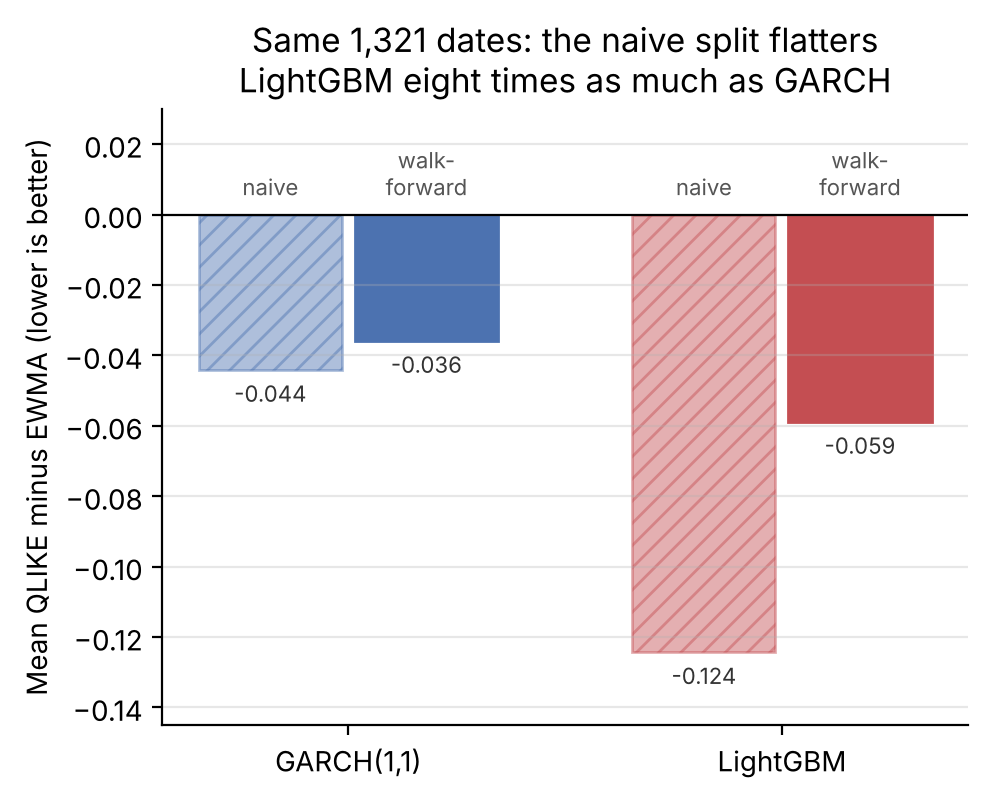
\includegraphics[width=0.55\textwidth,height=\textheight]{fig1_scheme_effect.png}
\caption{Mean QLIKE minus EWMA's on the 1,321 dates scored under both schemes (EWMA's forecasts are identical under both). The gap between each pair of bars is the scheme effect in Table 3.}
\end{figure}

\hypertarget{mechanism-the-forecast-ceiling-of-a-tree-ensemble}{%
\subsection{Mechanism: the forecast ceiling of a tree ensemble}\label{mechanism-the-forecast-ceiling-of-a-tree-ensemble}}

A boosted tree ensemble predicts by summing leaf values, and each leaf
value summarizes the training targets that reach it. Inputs beyond the
most extreme training inputs fall into the same boundary leaves, so the
forecast stops rising.

\textbf{The 2008 fold.} This model was trained on 1994 to late 2007. The
selected grid point was 31 leaves, at least 50 training dates per leaf and
L2 penalty 10, with 83 trees.

\begin{itemize}
\tightlist
\item
  The largest training target was 0.0099, about 70\% annualized
  volatility.
\item
  In the autumn of 2008 the model's inputs left that range. The 22-day
  realized variance reached 4.2 times its training maximum and was above
  it on 65 test dates. The 5-day Parkinson estimator reached 3.1 times its
  training maximum.
\item
  Realized 5-day variance exceeded the largest training target on 26 test
  dates. It peaked at 0.0352 (about 133\% annualized) for the forecast made
  on 2008-10-08.
\item
  On that date the model forecast 0.00216. Multiplying all eleven
  variance-type inputs by 2, 10 or 100 leaves the forecast at exactly
  0.00216.
\item
  The largest forecast this model makes on any date in the sample is
  0.00222, about 33\% annualized. That is well below even its own largest
  training target, because each leaf averages many training dates.
\end{itemize}

GARCH(1,1) has no such bound. Its forecast is linear in \(r_t^2\), and it
reached 0.0138 (about 83\% annualized) in the same weeks. That is still far
below realized variance, but six times the tree model's ceiling.

\begin{figure}
\centering
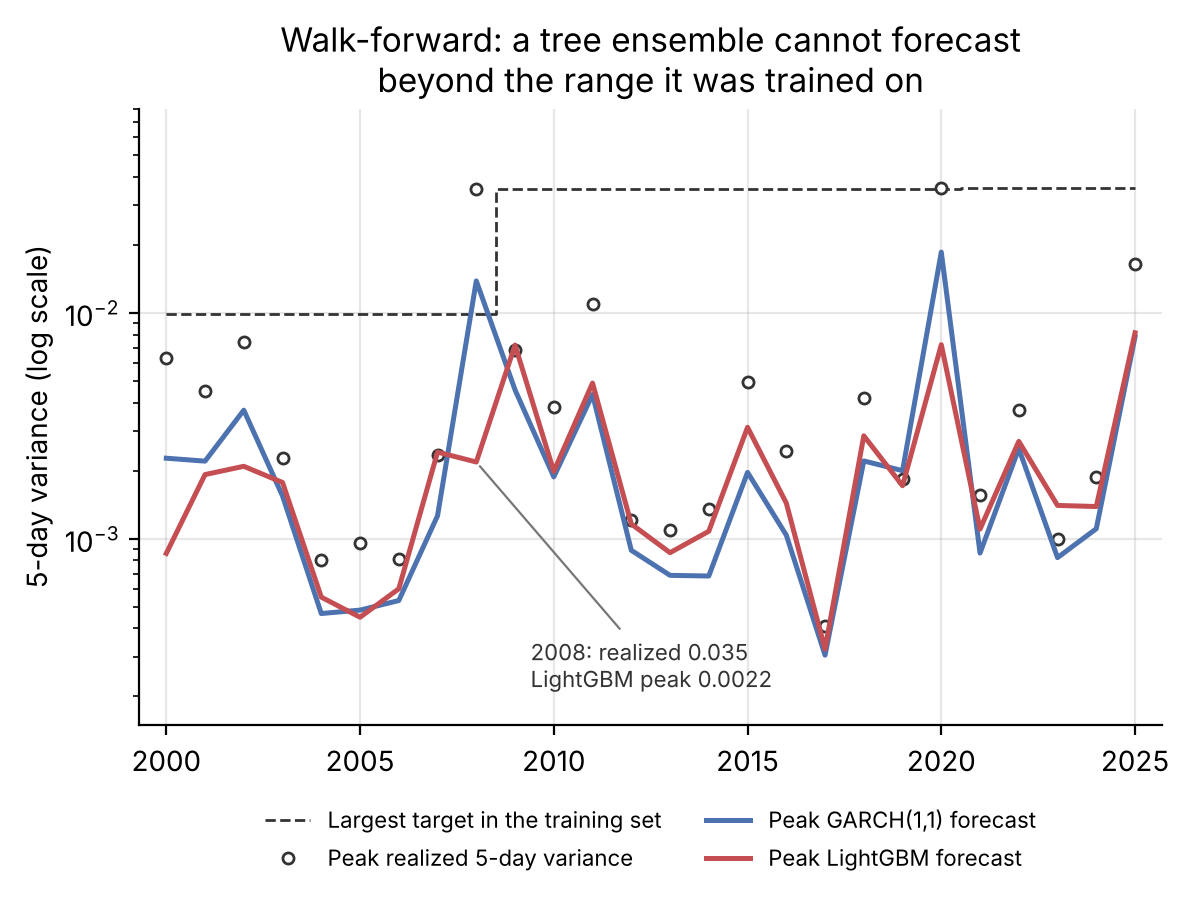
\includegraphics[width=0.75\textwidth,height=\textheight]{fig2_forecast_ceiling.png}
\caption{For each walk-forward test year: the largest target in that fold's training set (dashed), the peak realized 5-day variance (circles), and the peak forecast of GARCH(1,1) and LightGBM. Log scale.}
\end{figure}

\textbf{Consequence for the comparison.} In 2008 LightGBM's QLIKE is worse
than GARCH's by 0.70 per date. Averaged over all 6,534 dates, that one
year adds +0.027 to the mean difference, more than twice LightGBM's net
advantage of 0.012 (Appendix Table A1).

\begin{figure}
\centering
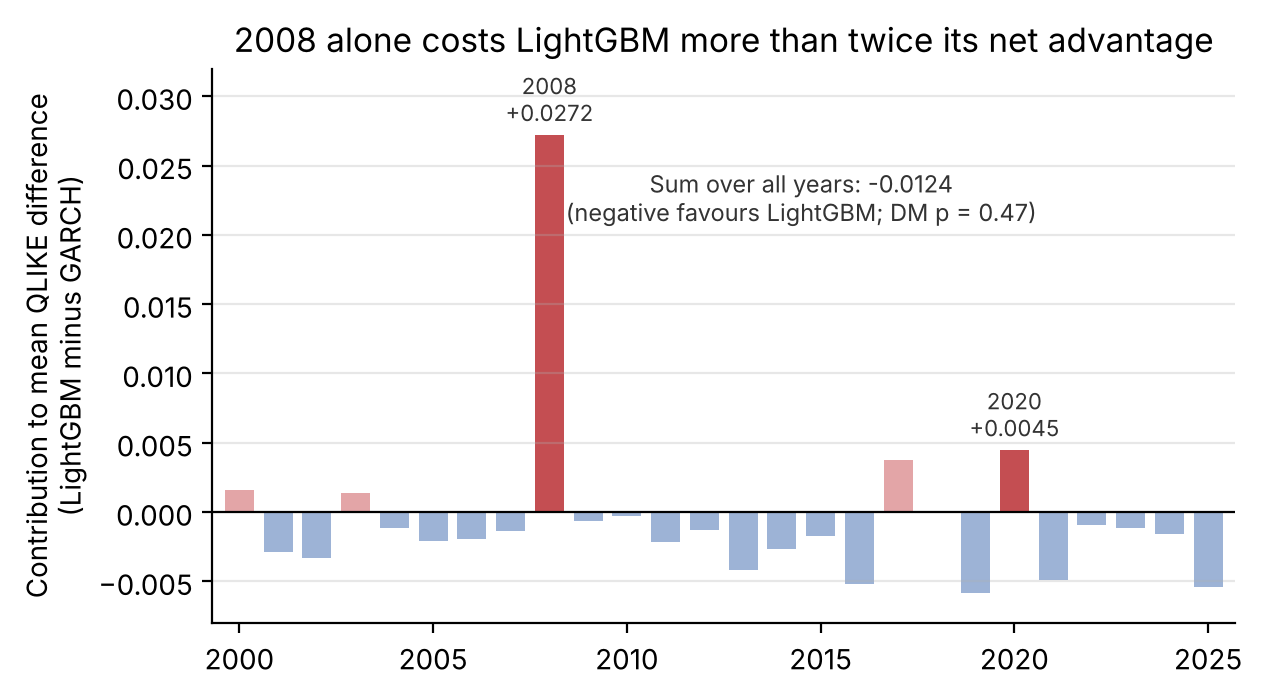
\includegraphics[width=0.75\textwidth,height=\textheight]{fig3_yearly_contribution.png}
\caption{Each year's contribution to the mean walk-forward QLIKE difference, LightGBM minus GARCH(1,1); the bars sum to −0.0124. Negative favours LightGBM. 2008 and 2020, the two years in which realized variance exceeded the training maximum, are highlighted.}
\end{figure}

\textbf{Other volatile years.} A consistent pattern appears across them. It was
examined after the results were known and is descriptive:

\begin{itemize}
\tightlist
\item
  \emph{Before 2008 was in training (the 2000--2008 folds):} LightGBM's largest
  forecast in any test year never exceeded 0.0024.
\item
  \emph{After 2008 entered training:} its peak forecasts reached 0.0072 (2009
  and 2020) and 0.0081 (2025).
\item
  \emph{Shocks within that range:} in 2011 (realized peak 0.0109) and 2025
  (0.0164), the peak LightGBM forecast matched or exceeded GARCH's, and
  LightGBM had the lower loss in both years.
\item
  \emph{A shock of 2008's size:} in 2020 (realized peak 0.0357), LightGBM's
  peak forecast was 0.0072 against GARCH's 0.0185, and it lost the year.
\end{itemize}

\hypertarget{why-qlike-and-rmse-disagree}{%
\subsection{Why QLIKE and RMSE disagree}\label{why-qlike-and-rmse-disagree}}

Under walk-forward, LightGBM has the best QLIKE and the worst RMSE. The two
losses weight different weeks.

\textbf{MSE is decided by the extremes.} The top 1\% of weeks by realized
variance (66 dates) account for 83\% of LightGBM's total squared error,
68\% of GARCH's and 65\% of EWMA's. LightGBM's mean forecast is 0.79 times
mean realized variance; GARCH's and EWMA's are 1.00. The shortfall sits in
the extreme weeks, where the ceiling binds.

\textbf{QLIKE scores relative errors.} Each week contributes on a comparable
scale, so the typical week dominates. On the remaining 99\% of dates
LightGBM's QLIKE is −6.724, against −6.686 for GARCH. Its RMSE there is
also the lowest, 6.5e-4 against 8.2e-4. This split is descriptive, not a
test.

\textbf{LightGBM is worse in the extreme weeks on both losses.} Its QLIKE in
the top 66 weeks is +1.05, against −1.38 for GARCH. But those weeks are 1\%
of the sample, and QLIKE averages over all weeks.

Year by year, LightGBM has the lower QLIKE in 21 of 26 years and the lower
MSE in 18. It is worse on QLIKE in 2000, 2003, 2008, 2017 and 2020.

\hypertarget{discussion}{%
\section{Discussion}\label{discussion}}

\textbf{The verdict.} By the pre-registered rule, the added complexity is \emph{not
justified}. LightGBM's walk-forward QLIKE advantage over GARCH(1,1) is not
statistically distinguishable from zero, and its RMSE is higher. This is
an absence of evidence for improvement, not evidence of equivalence. The
confidence interval admits a LightGBM advantage of up to about 0.046
QLIKE.

\textbf{When is complexity worth it?} The two steps up in complexity behaved
differently. Moving from EWMA to GARCH(1,1) adds three estimated
parameters. It buys a QLIKE improvement of 0.044 that holds at both lags.
That is consistent with mean reversion and an estimated reaction to shocks
describing index volatility well. Moving from GARCH to a flexible nonparametric model buys
a small, fairly consistent gain in ordinary conditions. It gives that gain
back when volatility leaves the range the model has seen, which is when a
volatility forecast matters most. GARCH's functional form extrapolates by
construction; a tree ensemble's does not.

\textbf{Why naive validation is especially misleading for flexible models.}
The naive split's bias scales with how much a model learns from individual
target rows. For a flexible model it hides the failure mode that decides
the out-of-sample comparison: a random split gives the model training
examples from the very crises it is later tested on.

\textbf{What might change the result.} Two kinds of design could remove the
ceiling: trees with linear leaves, or a model of RV relative to a GARCH
forecast rather than of RV itself. Either would let a flexible model
extrapolate. Neither was tried here, because doing so after seeing these
results would be the post-hoc redesign the study's protocol rules out.
They are hypotheses for a separate, pre-registered study.

\hypertarget{limitations}{%
\section{Limitations}\label{limitations}}

\begin{itemize}
\tightlist
\item
  \textbf{Scope.} The study covers one instrument, daily data, a 5-day horizon
  and 2000--2025 out of sample. The results say nothing directly about
  single stocks, other asset classes or intraday horizons.
\item
  \textbf{Proxy noise and power.} A sum of five squared daily returns is a
  noisy proxy for integrated variance. An intraday realized-variance
  target would rank the same forecasts more sharply and could narrow the
  confidence interval enough to be decisive.
\item
  \textbf{Two episodes dominate.} The net walk-forward comparison rests
  heavily on 2008 and 2020. The figures that exclude those years are
  descriptive, chosen after seeing the results, and are not evidence about
  calm markets.
\item
  \textbf{Information versus flexibility.} LightGBM saw the high--low range, the
  open and volume, which the baselines did not. It still showed no
  significant gain. No experiment separates the value of the extra inputs
  from the value of the model.
\item
  \textbf{One protocol.} The study used one ML configuration, one walk-forward
  scheme (expanding window, annual refits) and a symmetric GARCH baseline.
  A rolling window, more frequent refits or an asymmetric baseline might
  change the magnitudes.
\item
  \textbf{Naive-split tests.} The DM tests on the naive split treat the sorted
  random test dates as a time series. They are reported only as a
  contrast.
\item
  \textbf{Data.} \texttt{yfinance} is a free, unofficial source, and adjusted history
  can be revised. The recorded checksums make any such drift detectable.
\end{itemize}

\hypertarget{conclusion}{%
\section{Conclusion}\label{conclusion}}

Under proper walk-forward validation, a gradient-boosted tree model with
more information and a training loss matched to the evaluation metric did
not forecast SPY's weekly variance detectably better than GARCH(1,1). A
naive random split would have reported the opposite, with high confidence,
on both standard losses. The mechanism is concrete and measurable. A tree
ensemble cannot forecast beyond the targets it was trained on. The naive
split conceals this by training on the crises it tests. The lesson is
narrower than ``simple beats complex''. A flexible model's out-of-sample
value in volatility forecasting depends on whether it can extrapolate into
regimes it has not seen, and only a validation scheme that withholds those
regimes can tell.

\hypertarget{data-and-code-availability}{%
\section*{Data and code availability}\label{data-and-code-availability}}
\addcontentsline{toc}{section}{Data and code availability}

All code, tests, the design record (\texttt{DECISIONS.md}) and every recorded
output are available at
\url{https://github.com/mateeniqbal3/vol-forecast-model-comparison} under the
MIT License, and each release is archived on Zenodo (the DOI is listed in
the repository README). Raw prices are not redistributed; the data manifest
records checksums of the return series used. Appendix B lists the command
that regenerates each output. The figures are produced by
\texttt{python\ paper/make\_figures.py} from the committed result files only.

\hypertarget{acknowledgements-and-ai-use-disclosure}{%
\section*{Acknowledgements and AI-use disclosure}\label{acknowledgements-and-ai-use-disclosure}}
\addcontentsline{toc}{section}{Acknowledgements and AI-use disclosure}

AI tools (Claude, Anthropic) were used to assist with parts of the
software implementation and with drafting and editing this paper. All
research decisions, including the pre-registered design and decision rule,
were made and approved by the author, who takes full responsibility for
the content. Any errors are the author's own.

\hypertarget{references}{%
\section*{References}\label{references}}
\addcontentsline{toc}{section}{References}

\begin{list}{}{\setlength{\leftmargin}{1.5em}\setlength{\itemindent}{-1.5em}\setlength{\itemsep}{2pt}\setlength{\parsep}{0pt}}

\item Andersen, T. G., and Bollerslev, T. (1998). Answering the skeptics: Yes,
standard volatility models do provide accurate forecasts. \emph{International
Economic Review}, 39(4), 885--905.

\item Barndorff-Nielsen, O. E., Kinnebrock, S., and Shephard, N. (2010).
Measuring downside risk: Realised semivariance. In T. Bollerslev, J.
Russell and M. Watson (Eds.), \emph{Volatility and Time Series Econometrics:
Essays in Honor of Robert F. Engle}. Oxford University Press.

\item Bollerslev, T. (1986). Generalized autoregressive conditional
heteroskedasticity. \emph{Journal of Econometrics}, 31(3), 307--327.

\item Bollerslev, T., and Wooldridge, J. M. (1992). Quasi-maximum likelihood
estimation and inference in dynamic models with time-varying covariances.
\emph{Econometric Reviews}, 11(2), 143--172.

\item Christensen, K., Siggaard, M., and Veliyev, B. (2023). A machine learning
approach to volatility forecasting. \emph{Journal of Financial Econometrics},
21(5).

\item Corsi, F. (2009). A simple approximate long-memory model of realized
volatility. \emph{Journal of Financial Econometrics}, 7(2), 174--196.

\item Diebold, F. X., and Mariano, R. S. (1995). Comparing predictive accuracy.
\emph{Journal of Business \& Economic Statistics}, 13(3), 253--263.

\item Engle, R. F. (1982). Autoregressive conditional heteroscedasticity with
estimates of the variance of United Kingdom inflation. \emph{Econometrica},
50(4), 987--1007.

\item Friedman, J. H. (2001). Greedy function approximation: A gradient boosting
machine. \emph{Annals of Statistics}, 29(5), 1189--1232.

\item Glosten, L. R., Jagannathan, R., and Runkle, D. E. (1993). On the relation
between the expected value and the volatility of the nominal excess return
on stocks. \emph{Journal of Finance}, 48(5), 1779--1801.

\item Hansen, P. R., and Lunde, A. (2005). A forecast comparison of volatility
models: Does anything beat a GARCH(1,1)? \emph{Journal of Applied
Econometrics}, 20(7), 873--889.

\item J.P. Morgan and Reuters (1996). \emph{RiskMetrics --- Technical Document} (4th
ed.). New York.

\item Ke, G., Meng, Q., Finley, T., Wang, T., Chen, W., Ma, W., Ye, Q., and Liu,
T.-Y. (2017). LightGBM: A highly efficient gradient boosting decision
tree. \emph{Advances in Neural Information Processing Systems}, 30.

\item López de Prado, M. (2018). \emph{Advances in Financial Machine Learning}. Wiley.

\item Newey, W. K., and West, K. D. (1987). A simple, positive semi-definite,
heteroskedasticity and autocorrelation consistent covariance matrix.
\emph{Econometrica}, 55(3), 703--708.

\item Newey, W. K., and West, K. D. (1994). Automatic lag selection in
covariance matrix estimation. \emph{Review of Economic Studies}, 61(4),
631--653.

\item Parkinson, M. (1980). The extreme value method for estimating the variance
of the rate of return. \emph{Journal of Business}, 53(1), 61--65.

\item Patton, A. J. (2011). Volatility forecast comparison using imperfect
volatility proxies. \emph{Journal of Econometrics}, 160(1), 246--256.

\item Patton, A. J., and Sheppard, K. (2015). Good volatility, bad volatility:
Signed jumps and the persistence of volatility. \emph{Review of Economics and
Statistics}, 97(3), 683--697.

\end{list}

\appendix

\hypertarget{walk-forward-results-by-year}{%
\section{Walk-forward results by year}\label{walk-forward-results-by-year}}

\textbf{Table A1.} Δ is LightGBM minus GARCH(1,1); negative values favor
LightGBM. ``Training max RV'' is the largest target in that fold's training
set. The last column counts test dates whose realized RV exceeded it. The
yearly QLIKE differences, weighted by each year's share of dates, sum to
the full-sample difference of −0.0124.

\begin{longtable}[]{@{}
  >{\raggedright\arraybackslash}p{(\columnwidth - 16\tabcolsep) * \real{0.0682}}
  >{\raggedright\arraybackslash}p{(\columnwidth - 16\tabcolsep) * \real{0.0682}}
  >{\raggedright\arraybackslash}p{(\columnwidth - 16\tabcolsep) * \real{0.1364}}
  >{\raggedright\arraybackslash}p{(\columnwidth - 16\tabcolsep) * \real{0.1364}}
  >{\raggedright\arraybackslash}p{(\columnwidth - 16\tabcolsep) * \real{0.1136}}
  >{\raggedright\arraybackslash}p{(\columnwidth - 16\tabcolsep) * \real{0.1250}}
  >{\raggedright\arraybackslash}p{(\columnwidth - 16\tabcolsep) * \real{0.1136}}
  >{\raggedright\arraybackslash}p{(\columnwidth - 16\tabcolsep) * \real{0.1136}}
  >{\raggedright\arraybackslash}p{(\columnwidth - 16\tabcolsep) * \real{0.1250}}@{}}
\toprule\noalign{}
\begin{minipage}[b]{\linewidth}\raggedright
Year
\end{minipage} & \begin{minipage}[b]{\linewidth}\raggedright
n
\end{minipage} & \begin{minipage}[b]{\linewidth}\raggedright
QLIKE GARCH(1,1)
\end{minipage} & \begin{minipage}[b]{\linewidth}\raggedright
QLIKE LightGBM
\end{minipage} & \begin{minipage}[b]{\linewidth}\raggedright
Δ QLIKE
\end{minipage} & \begin{minipage}[b]{\linewidth}\raggedright
Δ MSE
\end{minipage} & \begin{minipage}[b]{\linewidth}\raggedright
Max realized RV
\end{minipage} & \begin{minipage}[b]{\linewidth}\raggedright
Training max RV
\end{minipage} & \begin{minipage}[b]{\linewidth}\raggedright
Dates above training max
\end{minipage} \\
\midrule\noalign{}
\endhead
\bottomrule\noalign{}
\endlastfoot
2000 & 252 & −5.7562 & −5.7141 & +0.0421 & +6.82e-08 & 0.0063 & 0.0099 & 0 \\
2001 & 248 & −5.9895 & −6.0661 & −0.0765 & −1.88e-07 & 0.0045 & 0.0099 & 0 \\
2002 & 252 & −5.6494 & −5.7347 & −0.0853 & −2.28e-07 & 0.0074 & 0.0099 & 0 \\
2003 & 252 & −6.6716 & −6.6361 & +0.0355 & +1.05e-08 & 0.0023 & 0.0099 & 0 \\
2004 & 252 & −7.2752 & −7.3041 & −0.0290 & −4.83e-09 & 0.0008 & 0.0099 & 0 \\
2005 & 252 & −7.4344 & −7.4884 & −0.0540 & −6.86e-09 & 0.0010 & 0.0099 & 0 \\
2006 & 251 & −7.5948 & −7.6459 & −0.0511 & −7.14e-09 & 0.0008 & 0.0099 & 0 \\
2007 & 251 & −6.5671 & −6.6035 & −0.0363 & +1.80e-08 & 0.0023 & 0.0099 & 0 \\
\textbf{2008} & 253 & −5.2103 & −4.5071 & \textbf{+0.7033} & \textbf{+1.34e-05} & 0.0352 & 0.0099 & \textbf{26} \\
2009 & 252 & −5.8550 & −5.8724 & −0.0173 & +6.90e-08 & 0.0068 & 0.0352 & 0 \\
2010 & 252 & −6.4879 & −6.4958 & −0.0079 & −2.99e-08 & 0.0038 & 0.0352 & 0 \\
2011 & 252 & −6.0699 & −6.1255 & −0.0556 & −1.51e-07 & 0.0109 & 0.0352 & 0 \\
2012 & 250 & −6.9905 & −7.0240 & −0.0335 & −1.65e-08 & 0.0012 & 0.0352 & 0 \\
2013 & 252 & −7.2833 & −7.3911 & −0.1078 & −1.64e-08 & 0.0011 & 0.0352 & 0 \\
2014 & 252 & −7.2837 & −7.3522 & −0.0685 & −9.81e-09 & 0.0014 & 0.0352 & 0 \\
2015 & 252 & −6.6611 & −6.7068 & −0.0457 & −4.30e-08 & 0.0049 & 0.0352 & 0 \\
2016 & 252 & −7.0385 & −7.1728 & −0.1343 & −2.65e-08 & 0.0025 & 0.0352 & 0 \\
2017 & 251 & −8.1022 & −8.0050 & +0.0972 & +8.35e-09 & 0.0004 & 0.0352 & 0 \\
2018 & 251 & −6.5094 & −6.5116 & −0.0022 & +7.82e-09 & 0.0042 & 0.0352 & 0 \\
2019 & 252 & −7.1429 & −7.2951 & −0.1521 & −6.65e-08 & 0.0018 & 0.0352 & 0 \\
\textbf{2020} & 253 & −5.6190 & −5.5030 & \textbf{+0.1160} & \textbf{+2.56e-07} & 0.0357 & 0.0352 & \textbf{3} \\
2021 & 252 & −6.9494 & −7.0769 & −0.1275 & −2.59e-08 & 0.0016 & 0.0357 & 0 \\
2022 & 251 & −5.7224 & −5.7469 & −0.0246 & −1.02e-07 & 0.0037 & 0.0357 & 0 \\
2023 & 250 & −7.0077 & −7.0379 & −0.0302 & −1.70e-09 & 0.0010 & 0.0357 & 0 \\
2024 & 252 & −7.0485 & −7.0893 & −0.0408 & −1.39e-08 & 0.0019 & 0.0357 & 0 \\
2025 & 245 & −6.5385 & −6.6831 & −0.1446 & −1.41e-06 & 0.0164 & 0.0357 & 0 \\
\end{longtable}

\hypertarget{reproducibility}{%
\section{Reproducibility}\label{reproducibility}}

Every number in this paper is produced by the repository's pipeline and
stored in version-controlled outputs. The exception is the stylized facts
in Section 3, which are printed by the executed EDA notebook
(\texttt{notebooks/01\_eda.ipynb}).

\needspace{18\baselineskip}
\begin{longtable}[]{@{}
  >{\raggedright\arraybackslash}p{(\columnwidth - 4\tabcolsep) * \real{0.3846}}
  >{\raggedright\arraybackslash}p{(\columnwidth - 4\tabcolsep) * \real{0.3269}}
  >{\raggedright\arraybackslash}p{(\columnwidth - 4\tabcolsep) * \real{0.2885}}@{}}
\toprule\noalign{}
\begin{minipage}[b]{\linewidth}\raggedright
Output
\end{minipage} & \begin{minipage}[b]{\linewidth}\raggedright
Command
\end{minipage} & \begin{minipage}[b]{\linewidth}\raggedright
Contents
\end{minipage} \\
\midrule\noalign{}
\endhead
\bottomrule\noalign{}
\endlastfoot
\texttt{data/dataset\_manifest.json} & \texttt{python\ -m\ src.data} & Sample, cleaning counts, return checksums \\
\texttt{docs/phase2\_naive\_baselines.json} & \texttt{python\ -m\ src.evaluate\ naive-baselines} & Baseline naive scores, recorded before the ML model existed \\
\texttt{docs/phase4\_validation\_results.json} & \texttt{python\ -m\ src.evaluate\ validate} & All models under both schemes; per-fold fitted parameters \\
\texttt{docs/phase5\_comparison.json} & \texttt{python\ -m\ src.evaluate\ compare} & Tables 1--3, A1; DM tests; ceiling probe; error concentration \\
\end{longtable}

The outputs are deterministic. Rerunning \texttt{validate} fails if the baseline
naive scores no longer match the record made before the ML model existed.
The test suite (92 tests, synthetic data) covers look-ahead freedom of the
target and of every feature, agreement of the GARCH filter with \texttt{arch},
the walk-forward split and purge, and the Newey--West variance against
\texttt{statsmodels}. The design record, including the configuration log and the
pre-registered decision rule, is in \texttt{DECISIONS.md}.

\end{document}
